%%%%%%%%%%%%%%%%%%%%%%%%%%%%%%%%%%%%%%%%%
% Short Sectioned Assignment
% LaTeX Template
% Version 1.0 (5/5/12)

%
% This template has been downloaded from:
% http://www.LaTeXTemplates.com
%
% Original author:
% Frits Wenneker (http://www.howtotex.com)
%
% License:
% CC BY-NC-SA 3.0 (http://creativecommons.org/licenses/by-nc-sa/3.0/)
%
%%%%%%%%%%%%%%%%%%%%%%%%%%%%%%%%%%%%%%%%%

%----------------------------------------------------------------------------------------
%	PACKAGES AND OTHER DOCUMENT CONFIGURATIONS
%----------------------------------------------------------------------------------------

\documentclass[paper=a4, fontsize=11pt]{scrartcl} % A4 paper and 11pt font size

\usepackage{graphicx} 
\usepackage{listings}
\usepackage[T1]{fontenc} % Use 8-bit encoding that has 256 glyphs
\usepackage{fourier} % Use the Adobe Utopia font for the document - comment this line to return to the LaTeX default
\usepackage[english]{babel} % English language/hyphenation
\usepackage{amsmath,amsfonts,amsthm} % Math packages
\usepackage{caption}
\captionsetup{font = {scriptsize}}
\usepackage{lipsum} % Used for inserting dummy 'Lorem ipsum' text into the template
\usepackage{subfigure}
\usepackage{latexsym}
\usepackage{sectsty} % Allows customizing section commands
\allsectionsfont{\centering \normalfont\scshape} % Make all sections centered, the default font and small caps
\usepackage{color} %red, green, blue, yellow, cyan, magenta, black, white
\definecolor{mygreen}{RGB}{28,172,0} % color values Red, Green, Blue
\definecolor{mylilas}{RGB}{170,55,241}
\usepackage{float}
\usepackage{fancyhdr} % Custom headers and footers
\pagestyle{fancyplain} % Makes all pages in the document conform to the custom headers and footers
\fancyhead{} % No page header - if you want one, create it in the same way as the footers below
\fancyfoot[L]{} % Empty left footer
\fancyfoot[C]{} % Empty center footer
\fancyfoot[R]{\thepage} % Page numbering for right footer
\renewcommand{\headrulewidth}{0pt} % Remo\label{\label{key}}ve header underlines
\renewcommand{\footrulewidth}{0pt} % Remove footer underlines
\setlength{\headheight}{13.6pt} % Customize the height of the header

\numberwithin{equation}{section} % Number equations within sections (i.e. 1.1, 1.2, 2.1, 2.2 instead of 1, 2, 3, 4)
\numberwithin{figure}{section} % Number figures within sections (i.e. 1.1, 1.2, 2.1, 2.2 instead of 1, 2, 3, 4)
\numberwithin{table}{section} % Number tables within sections (i.e. 1.1, 1.2, 2.1, 2.2 instead of 1, 2, 3, 4)
\newcommand{\mygamma}{\ensuremath{\gamma{}}}
\setlength\parindent{0pt} % Removes all indentation from paragraphs - comment this line for an assignment with lots of text

%----------------------------------------------------------------------------------------
%	TITLE SECTION
%----------------------------------------------------------------------------------------

\newcommand{\horrule}[1]{\rule{\linewidth}{#1}} % Create horizontal rule command with 1 argument of height

\title{	
\normalfont \normalsize 
\textsc{Purdue University} \\ [25pt] % Your university, school and/or department name(s)
\horrule{0.5pt} \\[0.4cm] % Thin top horizontal rule
\huge ECE 637 Laboratory Exercise 6 \\ 
\huge Introduction to Colorimetry\\% The assignment title
\horrule{2pt} \\[0.5cm] % Thick bottom horizontal rule
}

\author{Tong Shen} % Your name

\date{\normalsize\today} % Today's date or a custom date

\begin{document}

\maketitle % Print the title

%----------------------------------------------------------------------------------------
%	PROBLEM 1
%----------------------------------------------------------------------------------------
\section{Introduction}
Nothing to report for this section. 
\section{Plotting Color Matching Functions and Illuminants
}
In this section, we will plot the color matching functions and illuminants used in the laboratory

\begin{figure}[H]
	
	\centering
	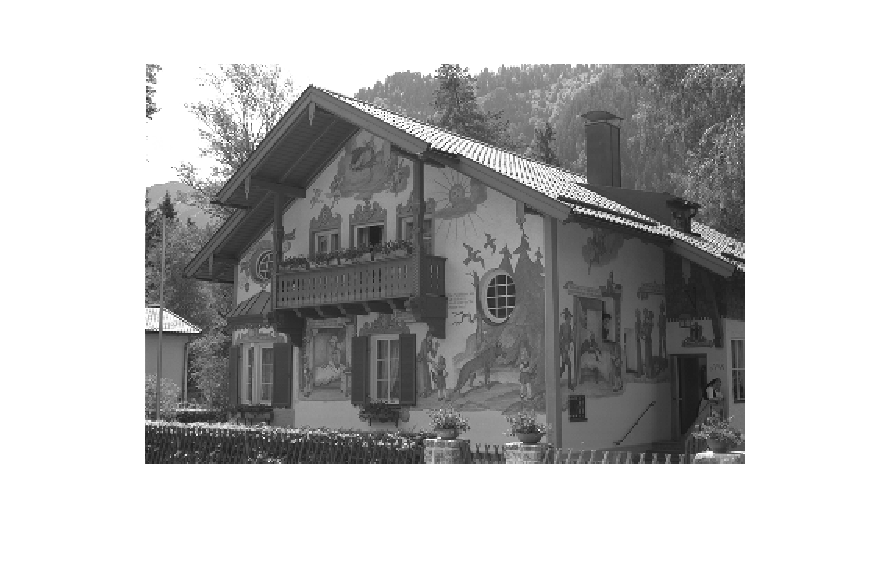
\includegraphics[height = 2.2in]{1.eps}
	\caption{The plot of the x$_0$($\lambda$), y$_0$($\lambda$), and z$_0$($\lambda$) color matching functions}
	
	
	
\end{figure}
\begin{figure}[H]
	
	\centering
	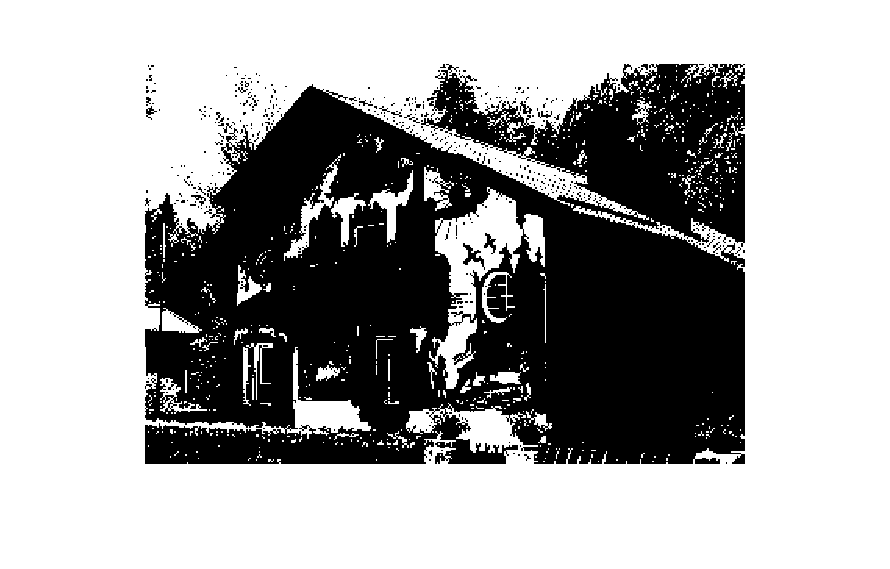
\includegraphics[height = 2.2in]{2.eps}
	\caption{The plot of the l$_0$($\lambda$), m$_0$($\lambda$), and s$_0$($\lambda$) color matching functions}
	
	
	
\end{figure}

\begin{figure}[H]
	
	\centering
	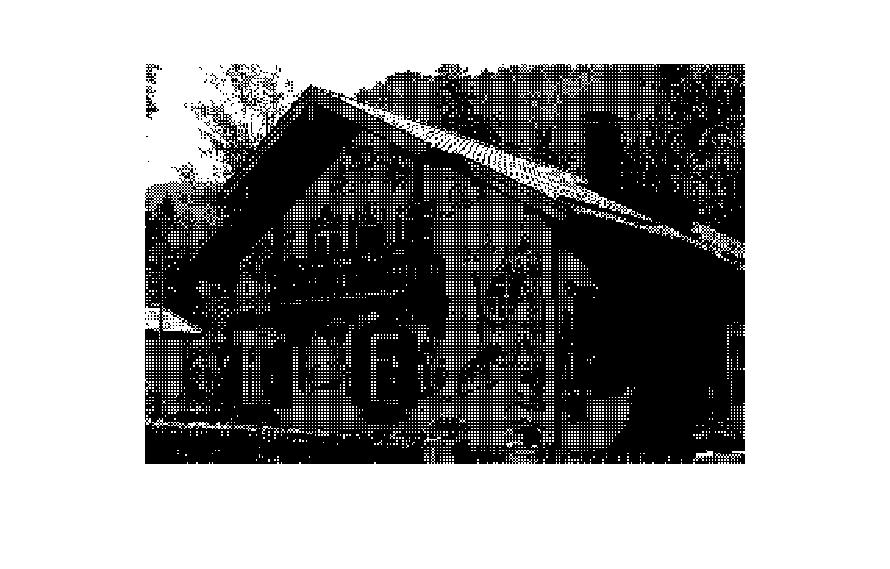
\includegraphics[height = 2.2in]{3.eps}
	\caption{The plot of the D$_{65}$ and fluorescent illuminants.}
	
	
	
\end{figure}
	
\section{ Chromaticity Diagrams}

A chromaticity diagram is a graphical representation of colors according to their position in
(x, y) chromaticity coordinates. Chromaticity coordinates have an important property that
combinations of any two colors always fall along a straight line between the two points. This
property will be useful in visualizing the structure of a color space.





%------------------------------------------------

\begin{figure}[H]
	
\centering
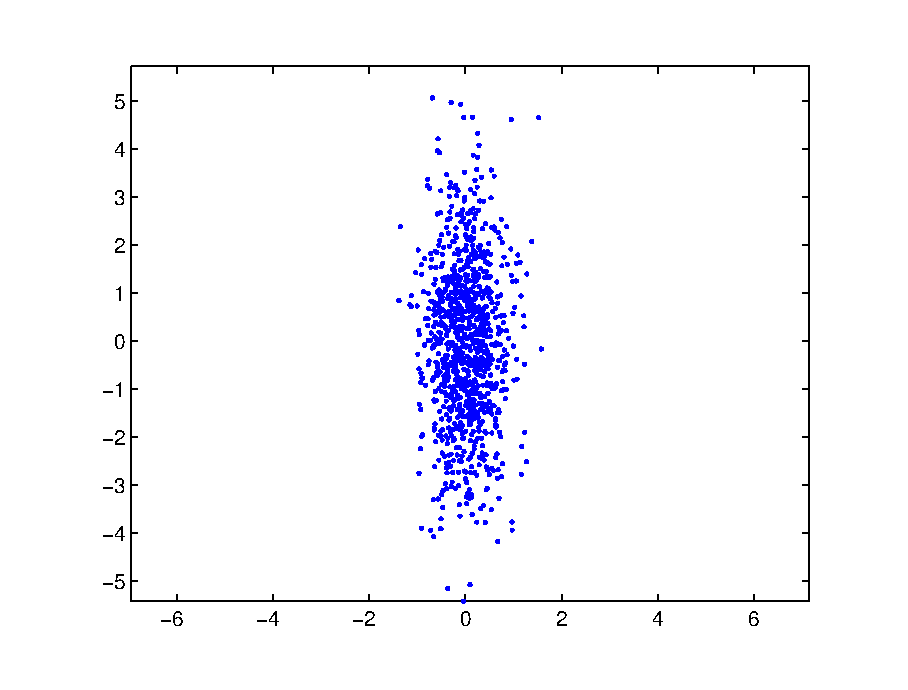
\includegraphics[height = 2.5in]{4.eps}
\caption{Labeled chromaticity diagram}
		
		
	
\end{figure}

\section{Rendering an Image from Illuminant, Reflectance,
	and Color Matching Functions
}
In this section, we will be to display a calibrated color image from a known illuminant
spectrum and the reflectance coefficients at each point in the image.


\vspace{6pt} 


The calculated matrix M$_{709-D65}$ is as follows:


\[
M_{709-D65} = 
\begin{bmatrix}
0.4124    &0.3576    &0.1805 \\
0.2126    &0.7152    &0.0722 \\
0.0193    &0.1192    &0.9505
\end{bmatrix}
\]

\begin{figure}[H]
	
	\centering
	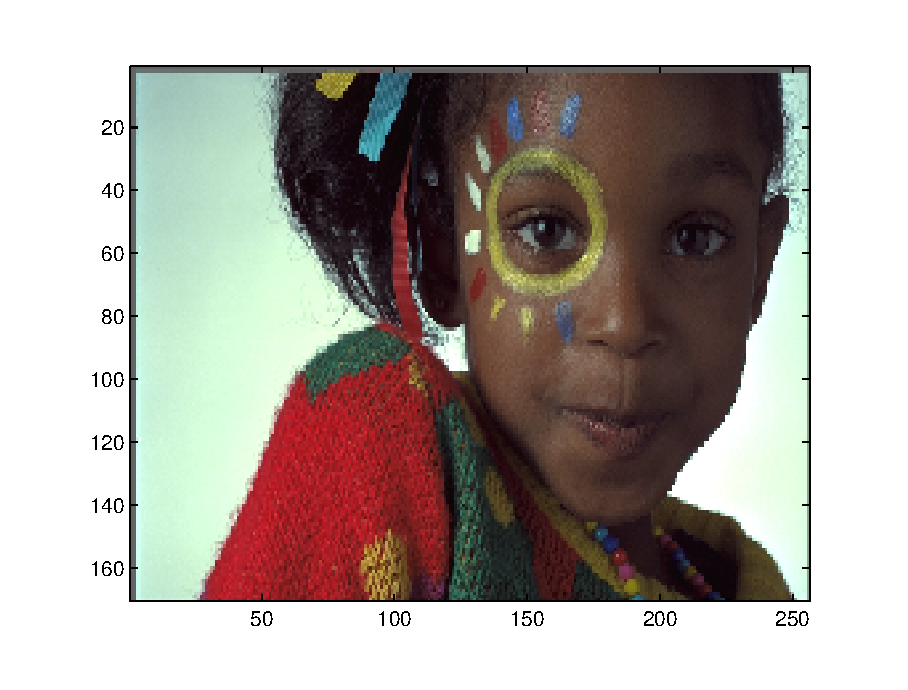
\includegraphics[height = 2.6in]{5.eps}
	\caption{Image obtained from D$_{65}$ light source}
	
	
	
\end{figure}

\begin{figure}[H]

\centering
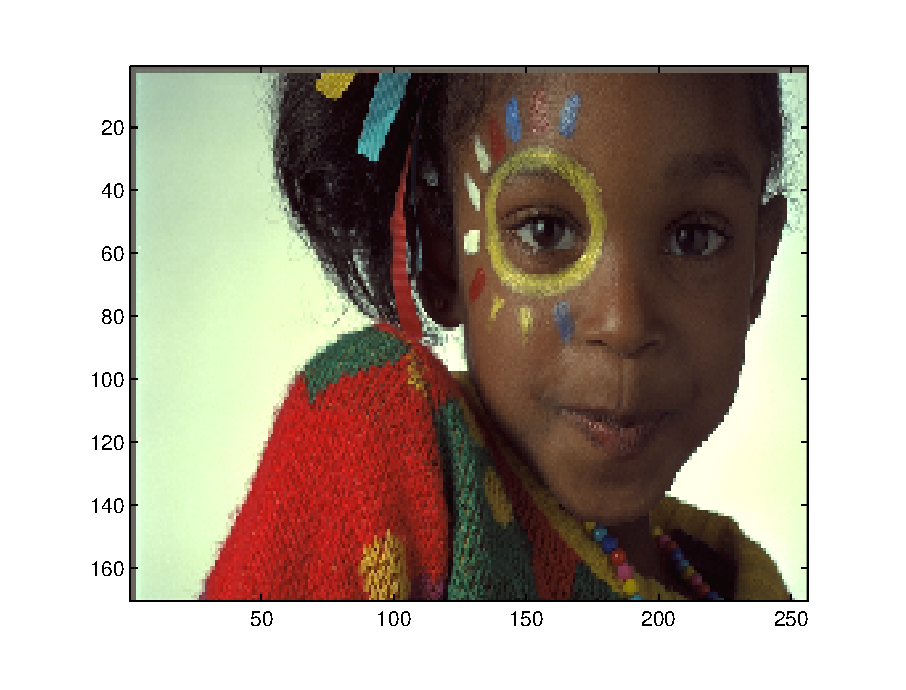
\includegraphics[height = 2.6in]{7.eps}
\caption{Image obtained from fluorescentc light source}

\end{figure}

According to the result, the image obtained from fluorescent light source is kind of bright and has more green color component. 

\section{Color Chromaticity Diagram}
In this exercise, we will create a chromaticity diagram similar to Section 3, but that will
also display a range of colors available from your monitor.

\begin{figure}[H]
	
	\centering
	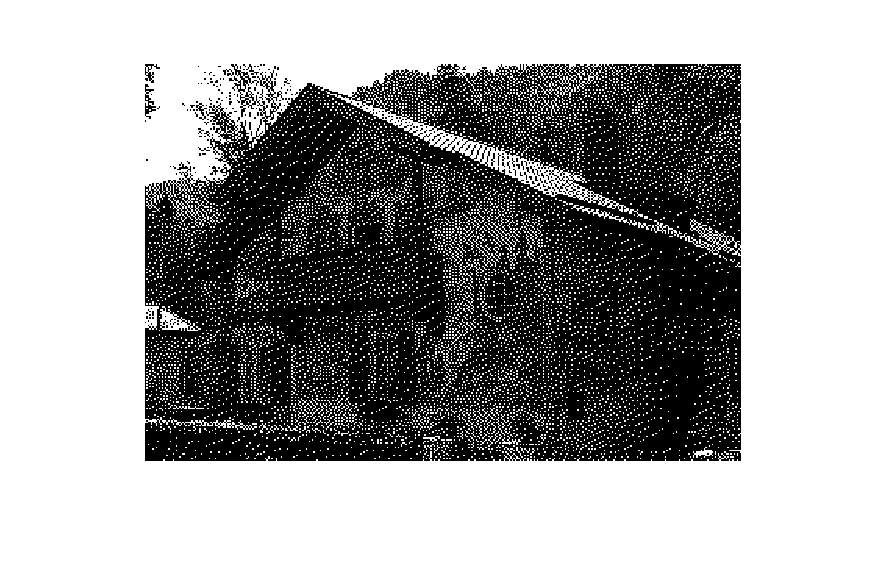
\includegraphics[height = 2.6in]{6.eps}
	\caption{Plot of the color diagram}
	
\end{figure}
\section{Code Listing}
\lstset{language=Matlab,%
	%basicstyle=\color{red},
	breaklines=true,%
	morekeywords={matlab2tikz},
	keywordstyle=\color{blue},%
	morekeywords=[2]{1}, keywordstyle=[2]{\color{black}},
	identifierstyle=\color{black},%
	stringstyle=\color{mylilas},
	commentstyle=\color{mygreen},%
	showstringspaces=false,%without this there will be a symbol in the places where there is a space
	numbers=left,%
	numberstyle={\tiny \color{black}},% size of the numbers
	numbersep=9pt, % this defines how far the numbers are from the text
	emph=[1]{for,end,break},emphstyle=[1]\color{red}, %some words to emphasise
	%emph=[2]{word1,word2}, emphstyle=[2]{style},    
}

\begin{lstlisting}[frame=single]



load('data.mat')

figure(1)
t = 400:10:700;
plot(t,[x;y;z])
legend('x_0(\lambda)','y_0(\lambda)','z_0(\lambda)')


A_inv = [0.2430 0.8560 -0.0440
-0.3910 1.1650 0.0870
0.0100 -0.0080 0.5630];
figure(2)
plot(t,A_inv*[x;y;z])
legend('l_0(\lambda)','m_0(\lambda)','s_0(\lambda)')


figure(3)
plot(t,[illum1;illum2])
legend('D_{65}','Fluorescence')

figure(4)
total = x + y + z;
plot(x./total,y./total)
hold on
CIE_1931 = [0.16658 0.00886 0.82456
0.73467 0.26533 0.0
0.27376 0.71741 0.00883
0.16658 0.00886 0.82456];

RGB_709 = [0.15 0.06 0.79
0.64 0.33 0.03
0.3 0.6 0.1
0.15 0.06 0.79];

plot(CIE_1931(:,1),CIE_1931(:,2),'r-')
text(CIE_1931(:,1),CIE_1931(:,2),'CIE_{1931}')

plot(RGB_709(:,1),RGB_709(:,2),'g-')
text(RGB_709(:,1),RGB_709(:,2),'RGB')

D_65 = [0.3127, 0.3290, 0.3583];
EE = [0.3333, 0.3333, 0.3333];

plot(D_65(1),D_65(2),'r*')
text(D_65(1),D_65(2),'D_{65}')

plot(EE(1),EE(2),'g*')
text(EE(1),EE(2),'EE')

orient tall
hold off
print('Chromaticity_diagram.tif')
%%%%%%%%%%%%%%%%%section 4
load('data.mat')
load('reflect.mat')
[sizeX sizeY sizeZ] = size(R);
I_1 = zeros([sizeX sizeY sizeZ]);
I_2 = zeros([sizeX sizeY sizeZ]);
for i = 1:sizeX
for j = 1:sizeY
for p = 1:sizeZ
I_1(i,j,p) = R(i,j,p)*illum1(p);
I_2(i,j,p) = R(i,j,p)*illum2(p);
end
end
end
XYZ_1 = zeros([sizeX sizeY 3]);
XYZ_2 = zeros([sizeX sizeY 3]);
for i = 1:sizeX
for j = 1:sizeY
XYZ_1(i,j,:) = permute(I_1(i,j,:),[2 3 1])*[x;y;z]';
XYZ_2(i,j,:) = permute(I_2(i,j,:),[2 3 1])*[x;y;z]';
end
end

RGB_709 = [0.64 0.33 0.03
0.3 0.6 0.1
0.15 0.06 0.79];
RGB_709 = RGB_709';
D_65_wp = [0.3127, 0.3290, 0.3583];
Wp = D_65_wp/D_65_wp(2);
k = inv(RGB_709)*Wp';
M = RGB_709*diag(k)

RGB_image_1 = zeros([sizeX sizeY 3]);
RGB_image_2 = zeros([sizeX sizeY 3]);
for i = 1:sizeX
for j = 1:sizeY
RGB_image_1(i,j,:) = inv(M) * permute(XYZ_1(i,j,:),[3 2 1]);  
RGB_image_2(i,j,:) = inv(M) * permute(XYZ_2(i,j,:),[3 2 1]);  
end
end

RGB_image_1(RGB_image_1 < 0) = 0;
RGB_image_1(RGB_image_1 > 1) = 1;
RGB_image_2(RGB_image_2 < 0) = 0;
RGB_image_2(RGB_image_2 > 1) = 1;

RGB_gamma1 = uint8(255*RGB_image_1.^(1/2.2));
RGB_gamma2 = uint8(255*RGB_image_2.^(1/2.2));
figure(5)
image(RGB_gamma1)
imwrite(RGB_gamma1,'illum1.tif')
figure(6)
image(RGB_gamma2)


%%%%%%%%%%%%%section 5

clc
clear
[x_c y_c] = meshgrid(0:0.005:1);
z = 1 - x_c - y_c;

RGB_709 = [0.64 0.33 0.03
0.3 0.6 0.1
0.15 0.06 0.79];
RGB_709 = RGB_709';

M = RGB_709;

[sizeX sizeY] = size(x_c);
XYZ = zeros(sizeX,sizeY,3);
XYZ(:,:,1) = x_c;
XYZ(:,:,2) = y_c;
XYZ(:,:,3) = z;

RGB_image = zeros(sizeX,sizeY,3);
for i = 1:sizeX
for j = 1:sizeY
RGB_image(i,j,:) = inv(M)*permute(XYZ(i,j,:),[3 2 1]);
if min(RGB_image(i,j,:)) < 0
RGB_image(i,j,:) = ones(3,1);
end
end
end


RGB_image(RGB_image < 0) = 1;

RGB_gamma = uint8(255*RGB_image.^(1/2.2));
figure(7)
image([0:0.005:1],[0:0.005:1],RGB_gamma)
axis('xy')
hold on

load('data.mat')
total = x + y + z;

plot(x./total,y./total)







\end{lstlisting}


\end{document}